\documentclass{article}
\usepackage{graphicx, soul}
\usepackage[dvipsnames]{xcolor}

\setul{0.5ex}{0.3ex}

\newcommand{\ulcolor}[2][Red]{\setulcolor{#1}\ul{#2}}
\newcommand*\sepline{%
  \begin{center}
    \rule[1ex]{.5\textwidth}{.5pt}
  \end{center}}

\title{Guía Práctica 2 - Comportamiento (Resuelto)}
\author{Juani Elosegui}
\date{Noviembre 2024}

\begin{document}
    
    \maketitle

    \section*{\underline{Ejercicio 1}}
        \textbf{Datos:}
        \\
        A: "esa persona muere en el próximo año"
        \\
        A$^{C}$: "esa persona NO muere en el próximo año"
        \\
        P(A) = 0,05; P(A$^{C}$) = 0,95
        \\
        \\
        \textbf{Planteo la forma normal:}
            \begin{table}[h]
                \begin{tabular}{ccc}
                    & Muere P(A) & No muere P(A$^{C}$) \\
                    Asegurar & -25.000; \ulcolor[Red]{0,05} & +100; \ulcolor[Red]{0,95} \\
                    No asegurar & 0; \ulcolor[Red]{0,05} & 0; \ulcolor[Red]{0,95} \\
                \end{tabular}
            \end{table}
        
        Si la persona muere y la aseguramos (ya cobramos $\$100$ de esa persona), entonces perdimos $\$25.000$. Conocemos la probabilidad de que muera y la probabilidad de que no muera. Si no aseguramos a la persona por tal razón, nos olvidamos, no ganamos ni perdemos plata.
        \\
        \\
        \textbf{Calculo el valor monetario esperado (EMV) si aseguramos o no aseguramos:}
        \\
        $EMV_{A}: -25.000 \cdot 0,05 + 100 \cdot 0,95 = -1.155$
        \\
        $EMV_{NA}: 0 \cdot 0,05 + 0 \cdot 0,95 = 0$
        \\
        \\
        \textbf{Conclusión:}
        \\
        Como $EMV_{NA} > EMV_{A}$, no nos conviene asegurar a la persona. Es más probable que perdamos plata.
        \\
        \\
        Si supiéramos con certeza que el individuo NO va a morir, lo podemos asegurar así cobramos los $\$100$ todos los años. Si sabemos que esta persona va a morir, no la vamos a asegurar, porque perderíamos mucha plata.
        \\
        El valor esperado con información perfecta es:
        \\
        $P(A) \cdot 100 + P(A^{C}) \cdot 0 = 95$.
        \\
        \\
        El precio de la información debería ser el valor esperado de la información perfecta menos el valor esperado con la información imperfecta:
        \\
        $\$95 - (-\$1.155) = \$1.250$

    \section*{\underline{Ejercicio 2}}
        \textbf{Datos:}
            \begin{itemize}
                \item La economía crece con una probabilidad de 0,5; se mantiene con una probabilidad de 0,3 y decrece con una probabilidad de 0,2.
                \item Los retornos son: $\$1.500$ en acciones y $\$900$ los bonos si la economía crece, $\$300$ en acciones y $\$600$ los bonos si la economía se mantiene, y se pierden $\$800$ en acciones y $\$200$ en bonos si la economía decrece.
                \item El plazo fijo nos da una ganancia de $\$500$ siempre, sin importar el estado de la economía.
            \end{itemize}
        \textbf{Forma normal:}
            \begin{table}[h]
                \begin{tabular}{cccc}
                                &            Crece              &           Mantiene            &         Decrece           \\
                    Acciones    & +1.500; \ulcolor[Green]{0,5}  & +300; \ulcolor[Yellow]{0,3}   & -800; \ulcolor[Red]{0,2}  \\
                    Bonos       & +900; \ulcolor[Green]{0,5}    & +600; \ulcolor[Yellow]{0,3}   & -200; \ulcolor[Red]{0,2}  \\
                    Plazo Fijo  & +500; \ulcolor[Green]{0,5}    & +500; \ulcolor[Yellow]{0,3}   & +500; \ulcolor[Red]{0,2}  \\
                \end{tabular}
            \end{table}
        \\
        \\
        \textbf{Calculo el valor monetario esperado (EMV) según en qué invirtamos:}
        \\
        $EMV_{A}: +1.500 \cdot 0,5 + 300 \cdot 0,3 - 800 \cdot 0,2 = \$680$
        \\
        $EMV_{B}: +900 \cdot 0,5 + 600 \cdot 0,3 - 200 \cdot 0,2 = \$530$
        \\
        $EMV_{PF}: +500 \cdot 0,5 + 500 \cdot 0,3 + 500 \cdot 0,2 = \$500$
        \\
        Como se puede ver, nos conviene invertir en acciones.
        \\
        \\
        \textbf{¿Cuánto tiene que valer el retorno del plazo fijo para que nos convenga invertir ahí?}
        \\
        Sea $x$ el retorno del plazo fijo.
        \\
        \\
        Necesitamos que se cumpla $EMV_{PF} \geq EMV_{A}$:
        \\
        $x \cdot 0,5 + x \cdot 0,3 + x \cdot 0,2 \geq \$680$
        \\
        $x \geq \$680$

    \section*{\underline{Ejercicio 3}}
        \textbf{Datos:}
        \\
        Costo de inversión: \$200.000
        \\
        El número de ventas dependerá del \textit{market share} de la empresa.
        \\
        Si el MS es pequeño, la empresa tendrá un ingreso de \$100.000; si es mediano, tendrá un ingreso de \$220.000; y, si es grande, tendrá un ingreso de \$350.000.
        \\
        P(MS pequeño) = 0,6; P(MS mediano) = 0,35; P(MS grande) = 0,05.
        \\
        \\
        \textbf{Árbol de decisión:}
        \begin{figure}[h]
            \centering
            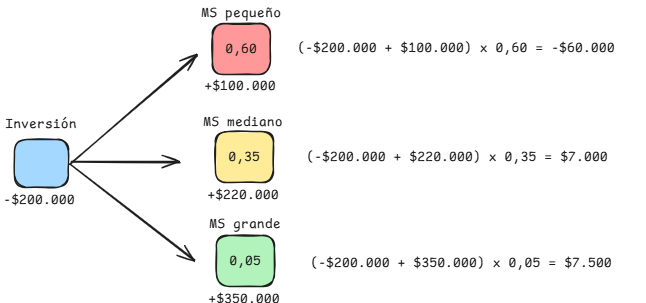
\includegraphics[width=0.8\linewidth]{figs/p3a.png}
        \end{figure}
        \\
        \\
        \textbf{Decisión:}
        \\
        No le conviene fabricar a la compañía, ya que perdería siempre básicamente.
        \\
        \\
        \textbf{¿Cuánto pagaría por la información?}
        \\
        $EV | PI = EMV | CI - EMV | SI$
        \\
        \\
        $EMV | SI  = (-200.000 + 100.000) \cdot 0,6 + (-200.000 + 220.000) \cdot 0.35 + (-200.000+350.000) \cdot 0,05$
        \\
        $EMV | SI = -\$45.500$
        \\
        \\
        $EMV | CI = (-\$200.000 + \$200.000) \cdot 0,6 + (-200.000 + 220.000) \cdot 0.35 + (-200.000+350.000) \cdot 0,05$
        \\
        $EMV | CI = \$0 \cdot 0,6 + \$20.000 \cdot 0.35 + \$150.000 \cdot 0.05$
        \\
        $EMV | CI = \$0 + \$7.000 + \$7.500$
        \\
        $EMV | CI = \$14.500$
        \\
        Acá, con la información perfecta, no produciríamos si sabemos que el MS nos da pérdidas. Es la mejor decisión: ¿por qué producirías si sabés que da pérdidas?
        \\
        \\
        $EV | PI = EMV | CI - EMV | SI$
        \\
        $EV | PI = \$14.500 - (-\$45.500)$
        \\
        $EV | PI = \$14.500 + \$45.500$
        \\
        $EV | PI = \$60.000$
        \\
        \\
        El máximo a pagar de la empresa por la información es $\$60.000$. Bastante más que la cometa que nos ofrecieron. Yo la pagaría.
    \section*{\underline{Ejercicio 4}}
        \textbf{Datos:}
        \\
        La máquina fabricada en Brasil sale \$1.100 y la fabricada en Argentina sale \$800.
        \\
        Si la máquina tuviese un problema, le saldría \$1.000 el arreglo.
        \\
        \\
        \textbf{Asumiendo que 2 de cada 10 laptops brasileras y 3 de cada 10 laptops argentinas vienen falladas, ¿cuánto estaría dispuesto a pagar Joaquín por información acerca de si le va a tocar una laptop fallada?}
        \\
        Ahora sabemos que P("se rompe una máquina brasilera") = 0,2 y P("se rompe una máquina argentina") = 0,3.
        \\
        \\
        Tengo que encontrar: EV$|$PI.
        \\
        \[EV|PI = EMV|CI - EMV|SI\]
        \[EV|PI = [(-\$1100 \cdot 0,8 + (-\$1100 -\$1000) \cdot 0,2)+(-\$800 \cdot 0,7 + (-\$800 -\$1000) \cdot 0,3] - [max\{.; .\}]\]
        \[EV|PI = [(-\$880 - (\$2.100) \cdot 0,2) + (-\$560 + (-\$1.800) \cdot 0,3)] - [max\{.; .\}]\]
        \[EV|PI = [(-\$880 - \$420) + (-\$560 -\$540)] - [max\{.; .\}]\]
        \[EV|PI = [(-\$1.300) + (-\$1.100)] - [\$-1.100]\]
        \[EV|PI = [-\$2.400] + [\$1.100]\]
        \[EV|PI = -\$3.300\]
        \textit{\ulcolor[Red]{La puta madre también. Me sigue dando negativo.}}
\\
    \sepline
    \section*{\underline{Ejercicio 1}}
        \textbf{Datos:}
        \\
        Para las acciones y los bonos, el retorno monetario depende de la economía. Para el plazo fijo no.
        \\
        \\
        Las probabilidades de que la economía crezca, se mantenga o disminuya son las siguientes. \(P($crece$) = 0.5, P($se mantiene$) = 0.3, P($baja$) = 0.2\).
        \\
        \\
        Los retornos son:
        \\
        \(R($acciones$ | $crece$) = +1.500, R($acciones$ | $se mantiene$) = +300, R($acciones$ | $disminuye$) = -8 v00\)
        \\
        \(R($bonos$ | $crece$) = +900, R($bonos$ | $se mantiene$) = +600), R($bonos$ | $disminuye$) = -200\)
        \\
        \\
        \textbf{¿Cuál es el mínimo valor de X para que convenga invertir en un plazo fijo siel inversor tiene una función de utilidad \((v)= \log_{2}(v+801)?\)}
        \\
        \\
        Para las acciones:
        \\
        Si la economía crece: \(u(1500) = \log_{2}(2301)\)
        \\
        Si la economía se mantiene: \(u(300) = \log_{2}(1101)\)
        \\
        Si la economía disminuye: \(u(-800) = \log_{2}(1)\)
        \\
        \(\Rightarrow \hat{u_{A}} \approx 0,5 \cdot u(1500) + 0,3 \cdot u(300) + 0,2 \cdot u(-800) \approx 8,62\)
        \\
        \\
        Para los bonos:
        \\
        Si la economía crece: \(u(900) = \log_{2}(1701)\)
        \\
        Si la economía se mantiene: \(u(600) = \log_{2}(1401)\)
        \\
        Si la economía disminuye: \(u(-200) = \log_{2}(601)\)
        \\
        \(\Rightarrow \hat{u_{B}} \approx 0,5 \cdot u(900) + 0,3 \cdot u(600) + 0,2 \cdot u(-200) \approx 10,24\)
        \\
        \\
        Para el plazo fijo:
        \\
        \(\Rightarrow \hat{u_{PF}} = \log_{2}(X+801)\)
        \\
        Ya que no depende del estado de la economía.
        \\
        \\
        Como se puede ver, \(\hat{u_{B}} > \hat{u_{A}}\). Esto hace que el inversionista prefiera invertir en bonos, ya que damos por supuesto que quiere generar la mayor utilidad posible.
        \\
        \\
        Para que el inversionista prefiera invertir en el plazo fijo, se debe cumplir que \(\hat{u_{PF}} > \hat{u_{B}}\):
        \\
        \[\log_{2}(X+801) > 10,24\]
        \[2^{\log_{2}(X+801)} > 2^{10,24}\]
        \[X+801 > 1209,34\]
        \[X > 408,34\]
        \\
        \\
        \textbf{¿Y cuánto debe valer X para que convenga invertir en el plazo fijo si su función es \((v)=(v+800)^{2}\)?}
        \\
        \\
        \(\hat{u_{A}} = 0,5 \cdot (2.300)^{2} + 0,3 \cdot (1.100)^{2} + 0,2 \cdot (0)^{2} \approx 300.800\)
        \\
        \(\hat{u_{B}} = 0,5 \cdot (1.700)^{2} + 0,3 \cdot (1.400)^{2} + 0,2 \cdot (600)^{2} \approx 2.105.000\)
        \\
        \\
        Como los bonos me generan más utilidad, el inversor elige invertir en ellos.
        \\
        \\
        \[\hat{u_{PF}} > \hat{u_{B}}\]
        \[(X+800)^{2} > 2.105.000\]
        \[X+800 > 1.450,86\]
        \[X > 650,86\]
    \section*{\underline{Ejercicio 2}}
        \textbf{Datos:}
        \\
        Se busca invertir 500 (millones) en República Previsible o Reino Caótico.
        \\
        \\
        Se sabe que el retorno de República Previsible es \(Ret(RP | $no crisis$) = +800\) y \(Ret(RP | $crisis$) = -500\).
        \\
        El retorno de Reino Caótico es \(Ret(RC | $no crisis$) = +1.500\) y \(Ret(RC | $crisis$) = -500\).
        \\
        \\
        La probabilidad de que República Previsible caiga en crisis es 0,2 y la probabilidad de que Reino Caótico lo haga es 0,5.
        \\
        \\
        \textbf{¿En qué país le conviene invertir a la empresa y cuál es el valor económico esperado de la decisión? Utilice EMVT para resolver este inciso del ejercicio.}
        \\
        Calculo el EMVT para los dos escenarios:
        \[\hat{RP}: 0,2 \cdot (-500) + 0,8 \cdot (800)\]
        \[\hat{RP}: -100 + 640\]
        \[\hat{RP}: 540\]
        \\
        \[\hat{RC}: 0,5 \cdot (-500) + 0,5 \cdot (1500)\]
        \[\hat{RC}: -250 + 750\]
        \[\hat{RC}: 500\]
        \\
        Conviene invertir en República Previsible porque su EMVT es mayor que el EMVT de Reino Caótico. \(\hat{RP} > \hat{RC}\).
        \\
        \\
        \textbf{Suponiendo que la empresa tiene una función de utilidad \(u(X) = (X + 500)^{\alpha}\), ¿Qué propiedad (¿mayor, menor o igual a qué?) debe cumplir \(\alpha\) para que la empresa tenga simpatía por el riesgo? Provea un ejemplo donde esto cambie la decisión del punto a.}
        \\
        \\
        Para que haya simpatía por el riesgo, \(\alpha\) debe ser positivo y par.
    \section*{\underline{Ejercicio 3}}
        \textbf{Datos:}
        \begin{itemize}
            \item Juan detecta intentos de fraude por internet. Su eficacia es del 99\%.
            \item La empresa le va a dar un bono si él hace que la empresa sufra 0 fraudes al año.
            \item Se sabe que la empresa sufre no menos de 500 intentos de fraude al año. En caso de haber exactamente 500 intentos y todos fallidos, le darán a Juan un bono de \$10.000.
        \end{itemize}
        \textbf{¿Qué formula debería usar la empresa para que el valor monetario esperado del bono sea constante en función del número de intentos detectados?}
        \\
        \\
        La fórmula será: \(10.000 - 20 \sum_{i = 0}^{500}S_{i} \cdot 0.01\)
        \\
        Sabemos que partimos de \$10.000 como máximo del bono que le pueden dar a Juan. Se restará \$20 por cada fraude -\(S_{i}\)- que Juan no puede erradicar (con una probabilidad del 0,01) de los 500 de los que se le presentan. Si erra todos, no percibe el bono. Si erradica a todos, percibe la totalidad del bono.
        \\
        \\
        \textit{\ulcolor[Red]{No sé si como MÁXIMO pueden haber 500 intentos de fraude. Fuente: Calibri (cuerpo)}}
    \section*{\underline{Ejercicio 4}}
        \textbf{Datos:}
        \begin{itemize}
            \item Carlos tiene una eficacia en detección de fraudes por internet del 99,5\% estimado en la primera prueba, y una eficacia menor -denominada $e$- en la segunda prueba. 
            \item La empresa piensa en mandarlo a Juan a fraudes telefónicos y ponerlo a Carlos en fraudes por internet.
            \item El problema es que se sabe en un 100\% que una de estas dos pruebas estuvo mal hecha. No se va a hacer una prueba más.
        \end{itemize}
        \textbf{Si el objetivo de la empresa es minimizar la chance que haya algún fraude, ¿debería cambiar de sector a Juan y Carlos? ¿Depende de $e$?}
        \\
        \[99 < \frac{99,5 \cdot 0,5 + e \cdot 0,5}{2}\]
        \[99 < \frac{49,75 + e \cdot 0,5}{2}\]
        \[99 < 22,875 + \frac{e}{4}\]
        Para que los cambien de área, la eficacia de Juan debe ser menor a la de Carlos. Se sabe que las dos pruebas que le hicieron a Carlos son equiprobables, y que la estimación de eficacia en las dos pruebas se determinan con un promedio.
        \\
        La decisión de la empresa de cambiarlos de área o no depende de la eficacia conseguida -$e$- en la segunda prueba de Carlos.
        \\
        \\
        \textbf{Si cada fraude no detectado le cuesta dinero a la empresa, ¿qué empleado es más costoso para la empresa en el largo plazo? ¿Depende de $e$?}
        \\
        \textit{Qué paja hacer esto. Intuitivamente diría que es más peligroso en cuanto a costos tenerlo a Carlos en fraudes por internet.}
\end{document}
